We apply a data-driven method~\cite{dyestnote} to estimate the $\dyll$ contributions in the 
same flavor $\ell^+\ell^-$ final states. This method also provides an estimate 
for the \emph{peaking component} of $WZ$ and $ZZ$ contributions, in which both 
leptons come from the same $Z$ boson.

The expected contributions from $\dyll$ events outside the $Z$-mass 
region in data can be estimated by counting the number of events near 
the $Z$ mass region in data, subtracting from it the non-$Z$ contributions, 
and scaling it by a ratio $R_{out/in}$ defined as the fraction of events outside and 
inside the $Z$-mass region in the simulation. The non-$Z$ contributions close to the 
$Z$-mass region in data is estimated from the number of events in the $e^\pm\mu^\mp$ final state 
$N_{in}^{e\mu}$, applying a correction factor that normalizes the 
electron-to-muon efficiency $k_{ee/\mu\mu}$. $R_{out/in}$ is obtained from simulation as 
$N_{out}^{MC}/N_{in}^{MC}$ with a looser $\met$ cut of 20 GeV (referred to as a loose selection). 
This method is described mathematically in Eq.~\ref{eq:dyest}. 
%%%%%%%%%%%%%%%%%%%%%%%%%%%%%%
\begin{eqnarray}
N_{out}^{ll,exp} = R_{out/in}^{ll,loose}(N_{in}^{ll} - 0.5N_{in}^{e\mu}k_{ll}), 
\label{eq:dyest}
\end{eqnarray}
%%%%%%%%%%%%%%%%%%%%%%%%%%%%%%
where $k_{ee} = \sqrt{\frac{N_{in}^{ee,loose}}{N_{in}^{\mu\mu,loose}}}$ for 
$\dyee$ and $k_{mm} = \sqrt{\frac{N_{in}^{\mu\mu,loose}}{N_{in}^{ee,loose}}}$ 
for $\dymm$. 
%To validate this method, we apply it first on events with no $\met$ cut. 
%These events are dominated by $\dyll$. A good agreement within 10\% between 
%the predictions from the data-driven method and simulation is observed. 

The method relies on the assumption that the dependence of the ratio $R_{out/in}$ 
on the $\met$ cut is well modelled by the simulation and is relatively flat. 
%An estimate of the degree to which this assumption fails is shown in  
Figure~\ref{fig:routin_met} shows the ratios $R_{out/in}$ as functions of 
the $\met$ cut at different jet bins determined from simulation.  
In the zero-jet bin, we have observed an increase of the 
ratio with respect to the $\met$ cut mainly due to the correlation of the 
$\met$ and the di-lepton mass measurement. The systematic uncertainty is assigned as the 
largest difference in the ratio to the central value as we vary the $\met$ cut from 
0 to 35 GeV. The results are tabulated in Table~\ref{tab:Routinmc}. 

We cross-checked the $R_{out/in}$ value in data. The idea is that all
background processes contribute equally to $ee$, $e\mu$, $\mu e$ and
$\mu\mu$ final states (after efficiency corrections), while Drell-Yan
only contributes to $ee$ and $\mu\mu$. Therefore we can subtract
$e\mu$ and $\mu e$ contribtutions from $ee$ and $\mu\mu$ ones to get
an estimate of Drell-Yan.
%as $$(N_{out}^{ll} - 0.5N_{out}^{e\mu}k_{ll})/(N_{in}^{ll} - 0.5N_{in}^{e\mu}k_{ll})$$. 
Figure~\ref{fig:routin_met_data} shows the dependence of $R_{out/in}$ of $\met$ cut evaluated 
in data. 


%%%%%%%%%%%%%%%%%%%%%%%%%%%%%%
\begin{table}
\begin{center}
\begin{tabular}{c c c }
\hline
\vspace{-3mm} && \\
Jet Bin & $R_{out/in}^{ee,loose}$ &  $R_{out/in}^{mm,loose}$\\
\vspace{-3mm} && \\
\hline
0 & 0.182 $\pm$ 0.013 $\pm$ 0.056 & 0.205 $\pm$ 0.011 $\pm$ 0.120 \\
1 & 0.160 $\pm$ 0.009 $\pm$ 0.020 & 0.167 $\pm$ 0.008 $\pm$ 0.010 \\
2 & 0.140 $\pm$ 0.017 $\pm$ 0.018 & 0.153 $\pm$ 0.015 $\pm$ 0.004 \\
\hline
\end{tabular}
\end{center}
\caption{The ratio $R_{out/in}^{ll,loose}$ at different jet bins evaluated from MC.  }
\label{tab:Routinmc}
\end{table}
%%%%%%%%%%%%%%%%%%%%%%%%%%%%%%

 %and gives the estimate of the systematic uncertainty
%of this background prediction. %The ratio $R_{out/in}$ is observed to be
%different for the dielectron and dimuon final states, as expected due to 
%the different $p_{T}$ cuts on the electron and muon candidates.



%%%%%%%%%%%%%%%%%%%%%%%%%%%%%%
\begin{figure}[!htbp]
\begin{center}
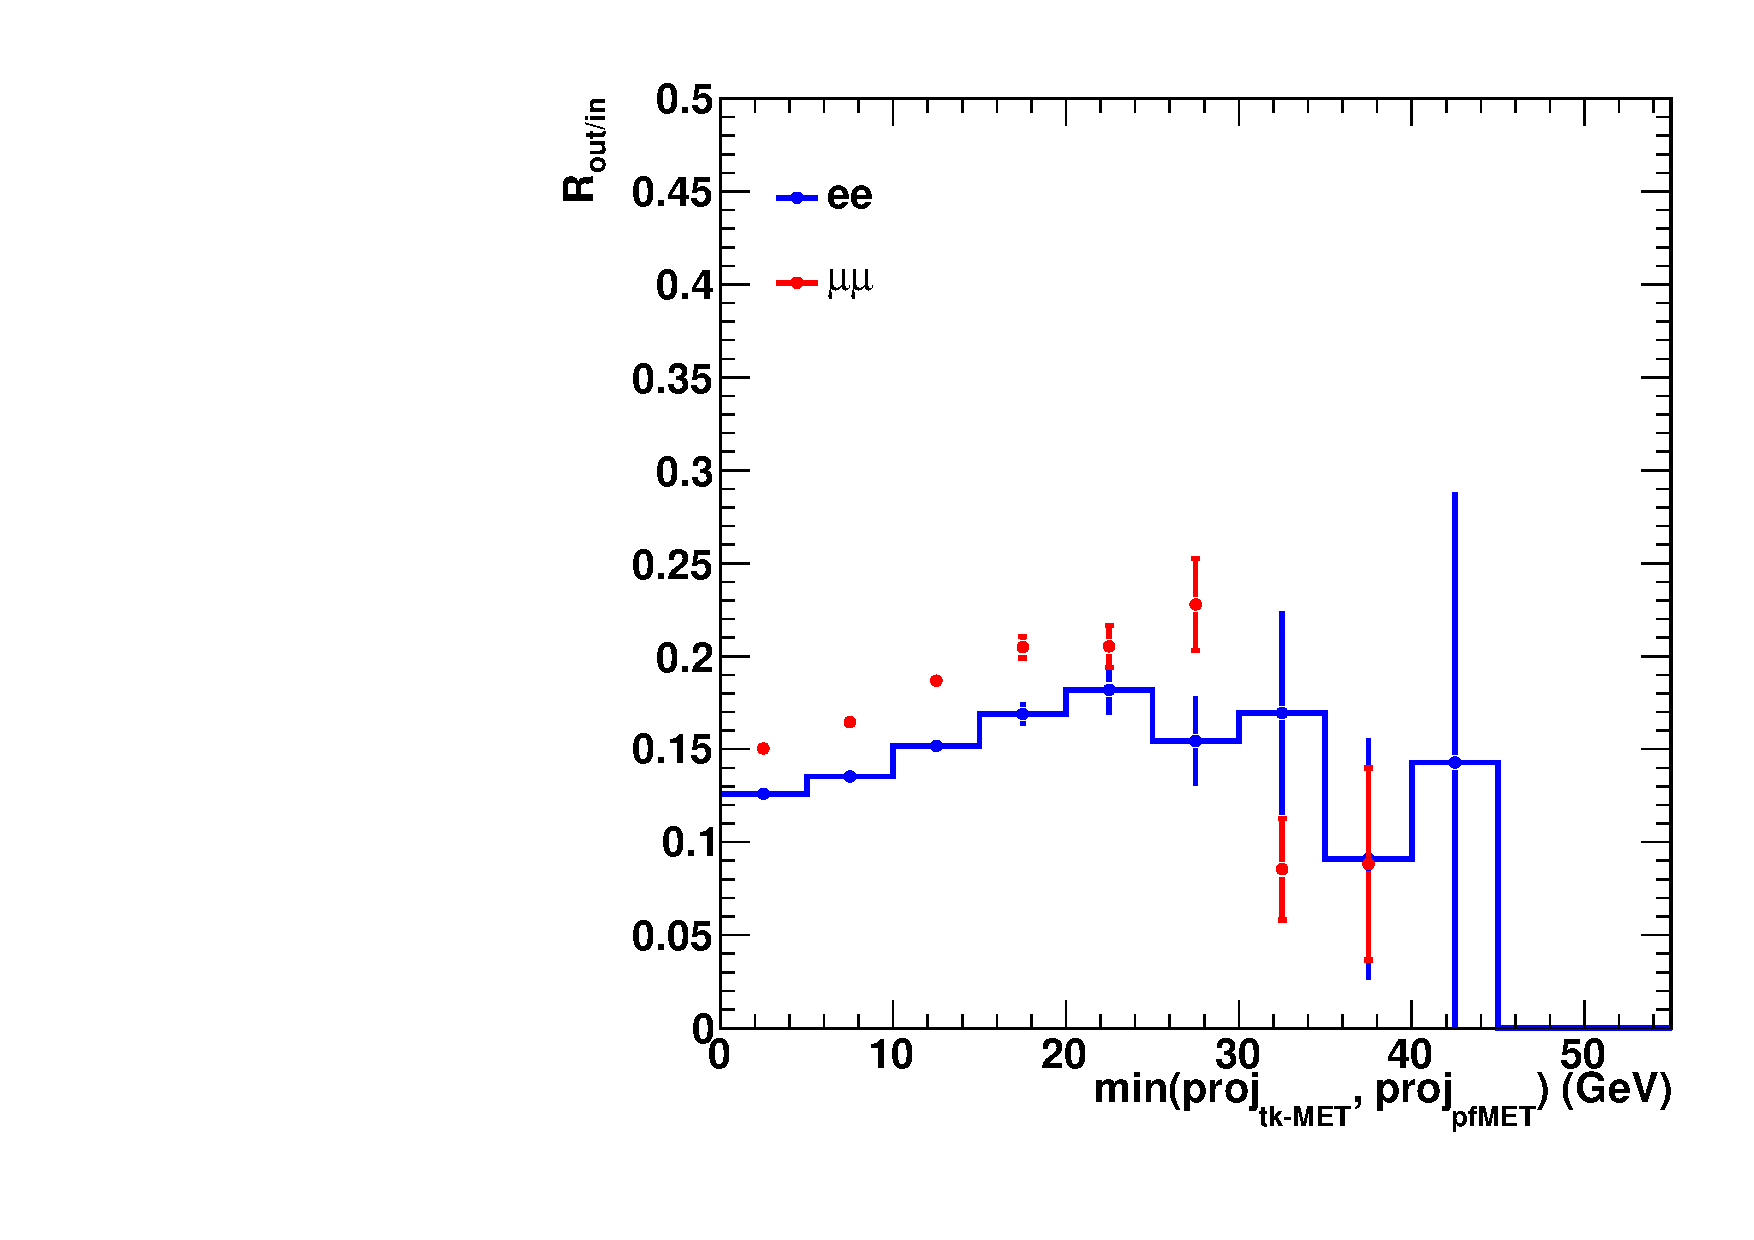
\includegraphics[width=0.3\textwidth]{figures/Routin_mc_0Jet.pdf}
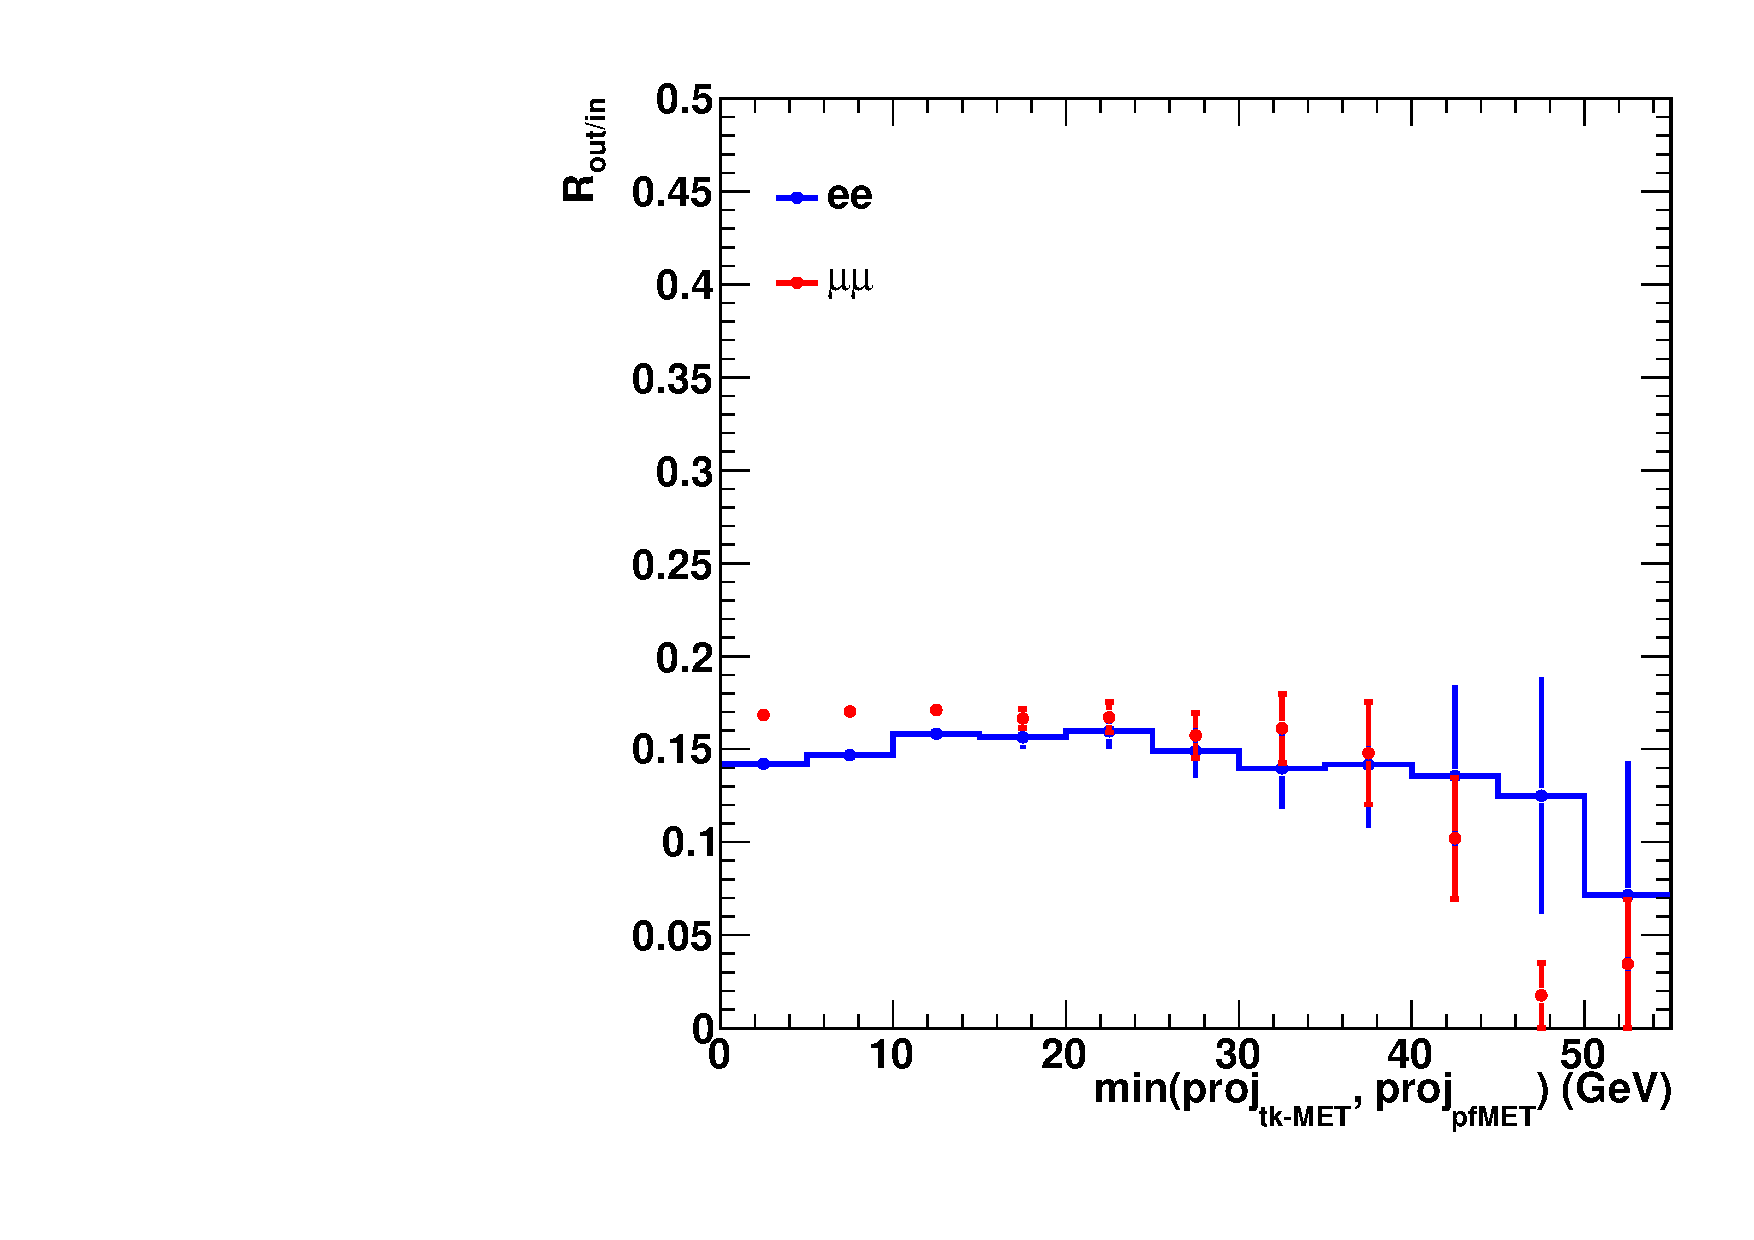
\includegraphics[width=0.3\textwidth]{figures/Routin_mc_1Jet.pdf}
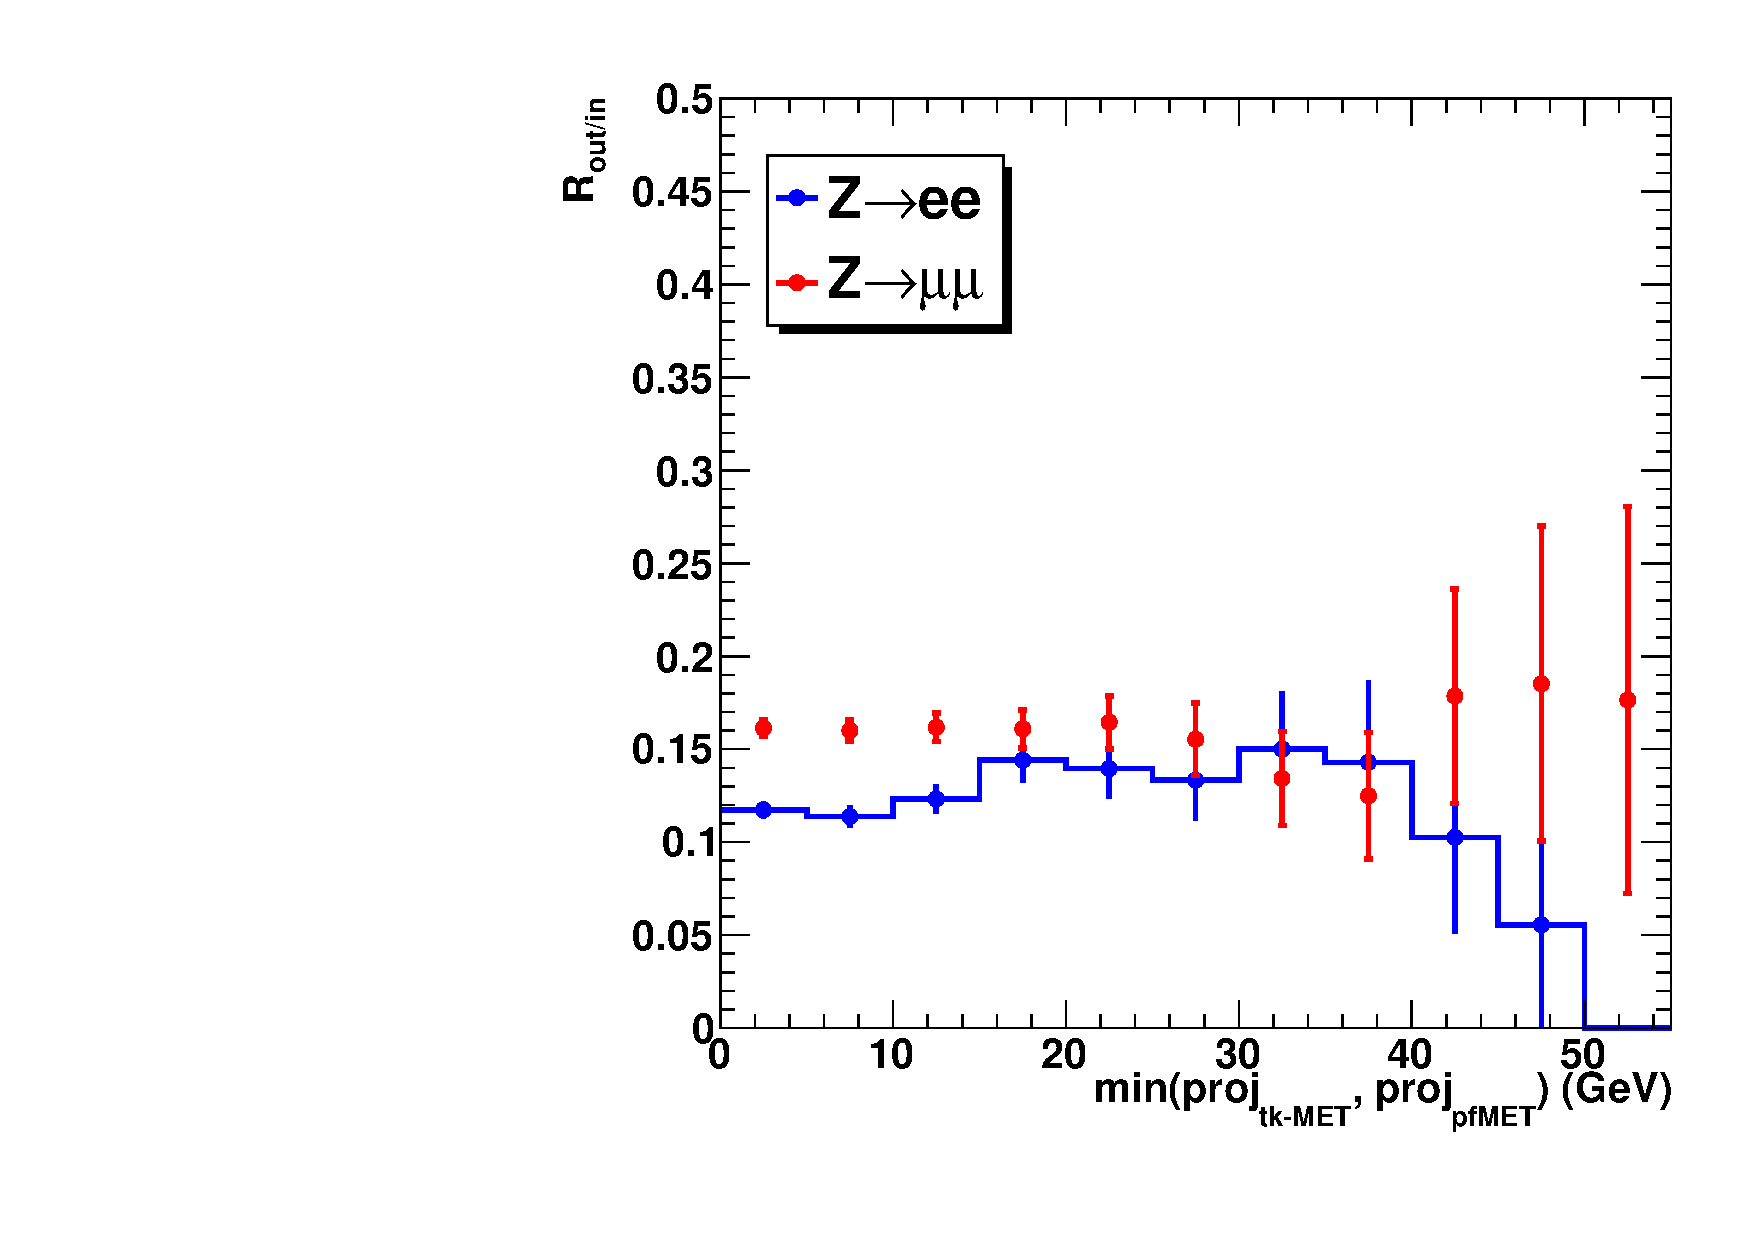
\includegraphics[width=0.3\textwidth]{figures/Routin_mc_2Jet.pdf}
\caption{ The ratio $R_{out/in}$ as a function of the $\met$ cut obtained using MC in the 
0-Jet (left), 1-Jet (middle) and 2-Jet (right) bins.} %The difference in the ratio between 
%\ee\ and \mm\ final states is due to lower minimum muon momentum compared with electron
%(10 GeV vs 15 GeV), which allows for more low mass Drell-Yan events.}
\label{fig:routin_met}
\end{center}
\end{figure}
%%%%%%%%%%%%%%%%%%%%%%%%%%%%%%


%%%%%%%%%%%%%%%%%%%%%%%%%%%%%%
\begin{figure}[!htbp]
\begin{center}
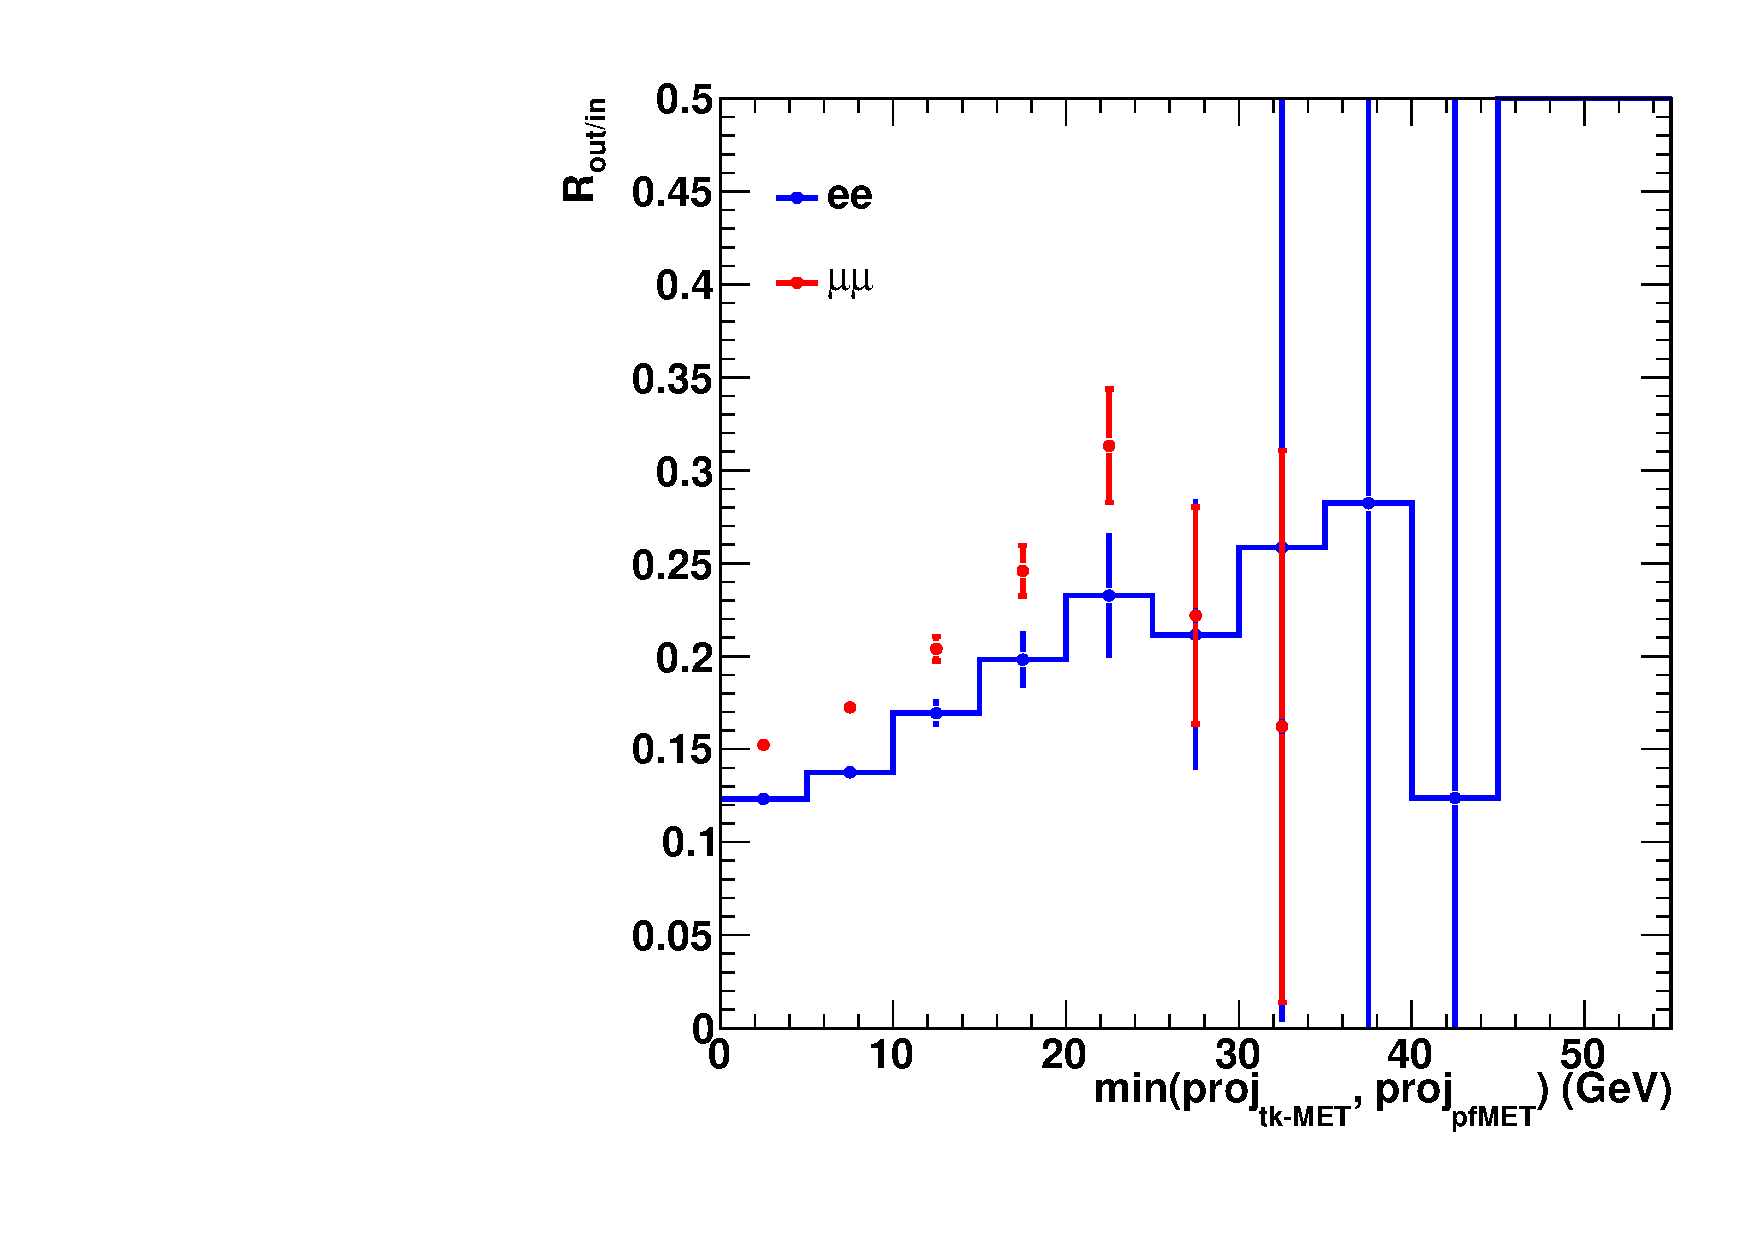
\includegraphics[width=0.3\textwidth]{figures/Routin_data_0Jet.pdf}
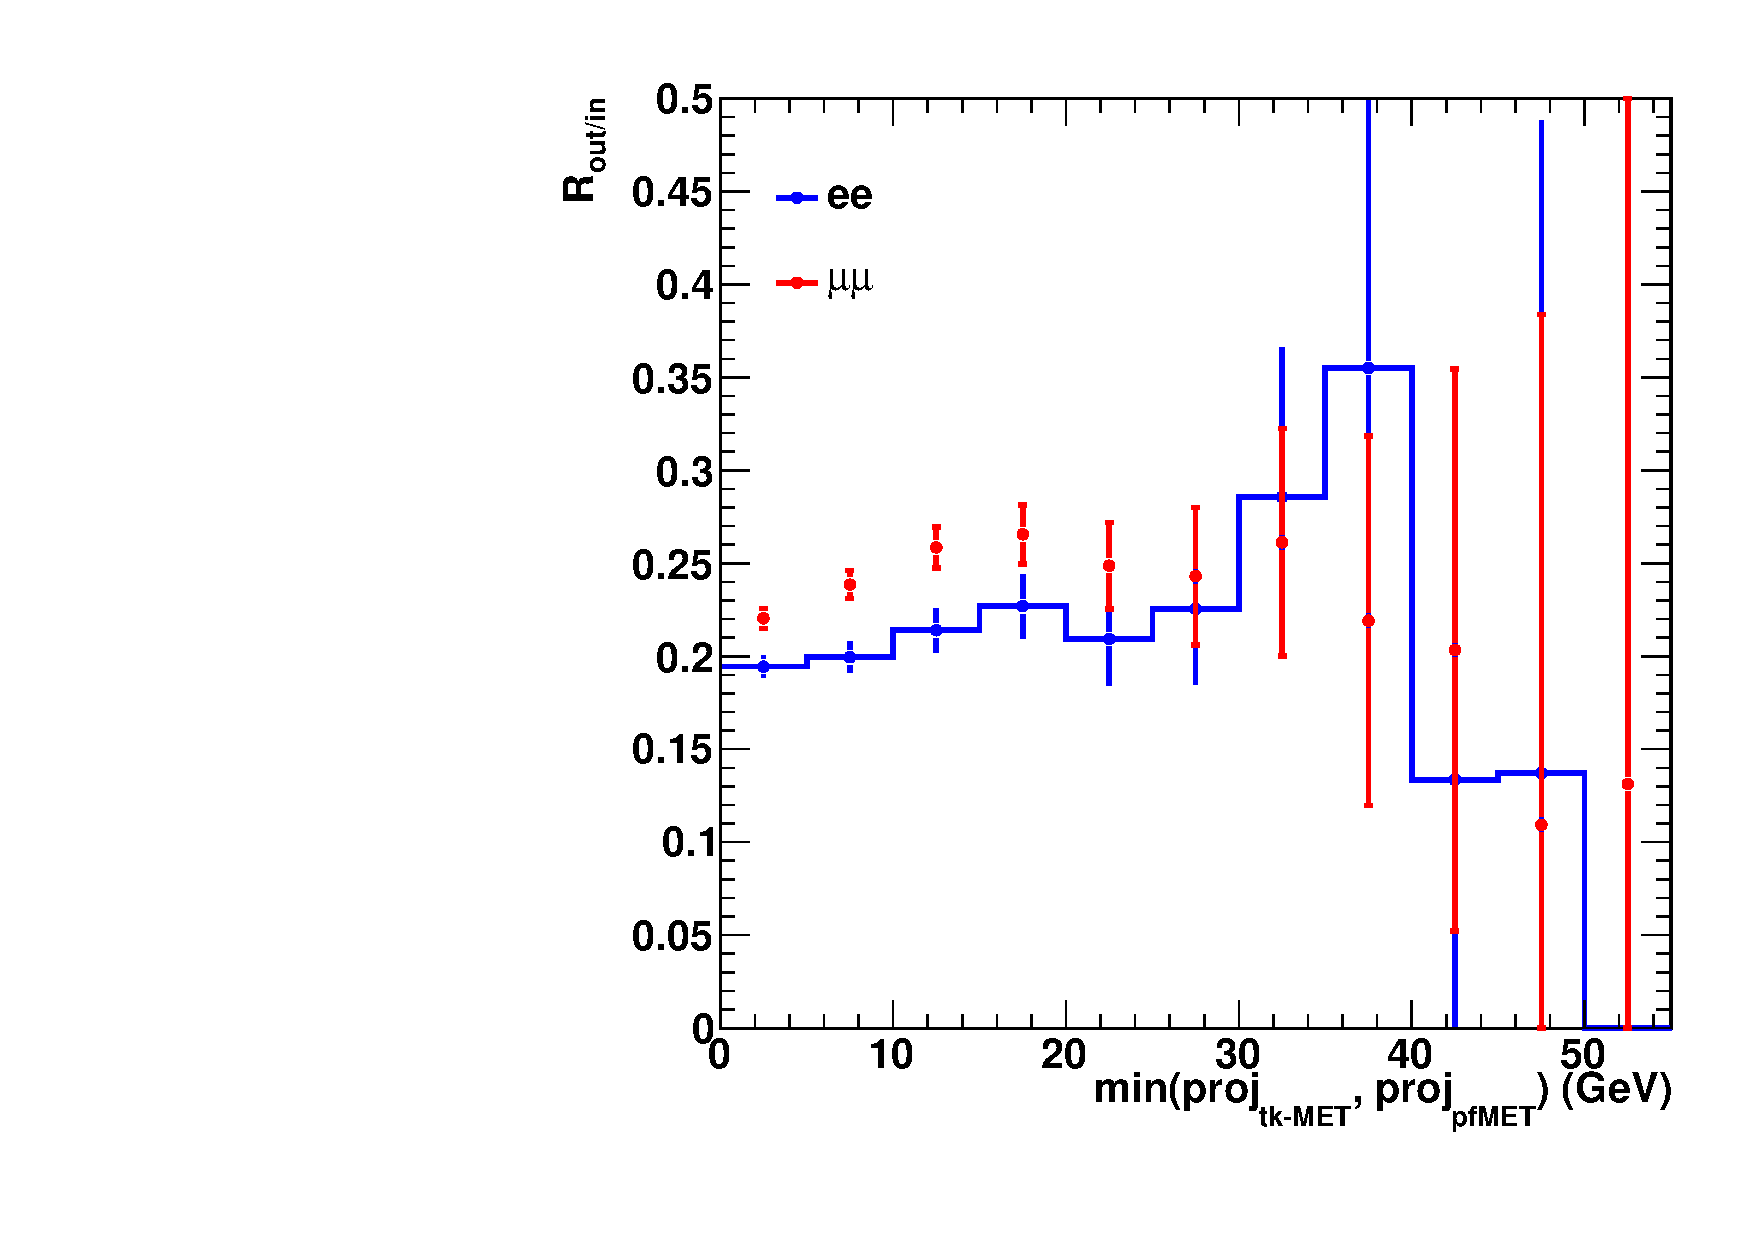
\includegraphics[width=0.3\textwidth]{figures/Routin_data_1Jet.pdf}
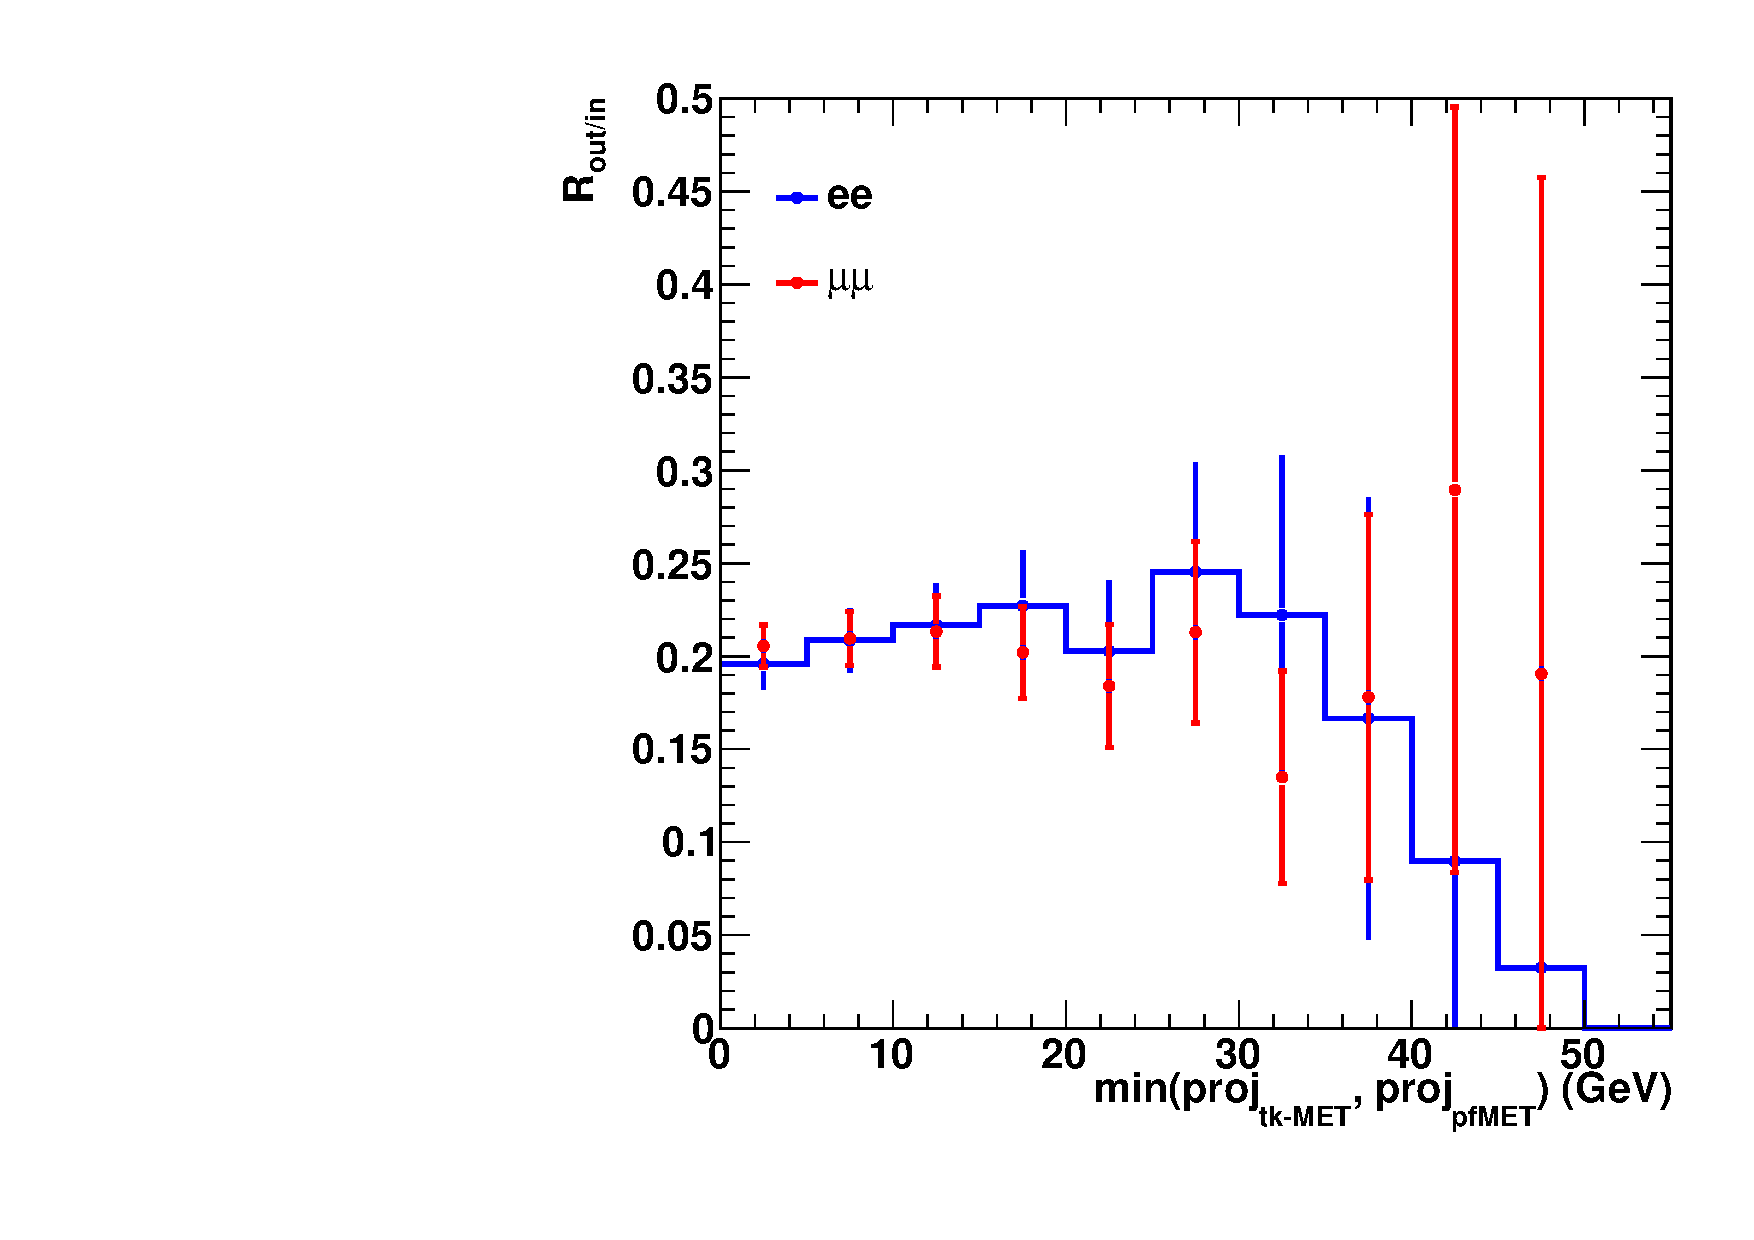
\includegraphics[width=0.3\textwidth]{figures/Routin_data_2Jet.pdf}
\caption{ The ratio $R_{out/in}$ as a function of the $\met$ cut obtained from data in the 
0-Jet (left), 1-Jet (middle) and 2-Jet (right) bins.} %The difference in the ratio between 
%\ee\ and \mm\ final states is due to lower minimum muon momentum compared with electron
%(10 GeV vs 15 GeV), which allows for more low mass Drell-Yan events.}
\label{fig:routin_met_data}
\end{center}
\end{figure}
%%%%%%%%%%%%%%%%%%%%%%%%%%%%%%
